The following two chapters consider the impact of using emerging NVRAM technologies for durable transaction processing.
Refer to Section~\ref{sec:Background:Storage:NVRAM} for an overview of storage technologies and Section~\ref{sec:Background:Recovery} for a description of ARIES, a popular recovery mechanism for disk.
The work presented in these two chapters was originally published in VLDB 2014 \cite{Pelley13}.
I completed this work under the guidance of my advisor, Thomas F. Wenisch, and collaborators at Oracle, Brian T. Gold and Bill Bridge.
I would especially like the thank Brian and Bill for bringing industry's point of view and ``real world" examples to this collaboration.
This chapter outlines the problems with existing disk recovery management, the potential pitfalls of using NVRAM for persistent applications, a methodology for evaluating NVRAM devices that are not yet available, and a description of several candidate software designs for NVRAM recovery management, to be evaluated in the next chapter.

\section{Introduction}
\label{sec:OLTP_design:Intro}

Emerging nonvolatile memory technologies (NVRAM) offer an alternative to disk that is persistent, provides read latency similar to DRAM, and is byte-addressable \cite{BurrKurdi08}.
Such NVRAMs could revolutionize online transaction processing (OLTP), which today must employ sophisticated optimizations with substantial software overheads to overcome the long latency and poor random access performance of disk.
Nevertheless, many candidate NVRAM technologies exhibit their own limitations, such as greater-than-DRAM latency, particularly for writes \cite{LeeIpek09}.

These NVRAM technologies stand to revolutionize Online Transaction Processing (OLTP), where consistency and durability are paramount, but applications demand high throughput and low latency.
Prior work has already demonstrated the potential of these technologies to enhance file systems \cite{ConditNightingale09} and persistent data structures \cite{VenkataramanTolia11}, but has not considered OLTP.
Today, OLTP systems are designed from the ground up to circumvent disk's performance limitations.
For example, many popular database systems use Write-Ahead Logging (WAL; e.g., ARIES \cite{MohanHaderle92}) to avoid expensive random disk writes by instead writing to a sequential log.  
Although effective at hiding write latency, WAL entails substantial software overheads.

NVRAM offers an opportunity to simultaneously improve database transaction processing throughput and recovery latency by rethinking mechanisms that were designed to address the limitations of disk.
Figure~\ref{fig::Recovery} demonstrates this potential, displaying recovery time and transaction throughput for the TPCB workload running on the Shore-MT storage manager \cite{JohnsonPandis09} for hypothetical NVRAM devices (see Section~\ref{sec:OLTP_design:Methodology} for a description of the methodology).

\begin{figure}
  \centering
  \includegraphics[width=.7\linewidth]{OLTP_design/TPCB_Recovery.pdf}
  \caption{\textbf{TPCB recovery latency vs throughput.} Increasing page flush rate reduces recovery latency.  Removing WAL entirely improves throughput by 50\%.}
  \label{fig::Recovery}
\end{figure}


The ARIES/WAL points (black circles) in the Figure show forward-processing throughput (horizontal axis) and recovery time (vertical axis) as a function of device write throughput (annotated alongside each point as pages per second).
As database throughput can greatly outpace existing storage devices (this configuration requires 6,000 page writes/s to bound recovery; measured disk and flash devices provide only 190 and 2,500 page writes/s, respectively) I model recovery performance under faster NVRAM using a RAM disk for log and heap while limiting the page flush rate.
As intuition would suggest, greater write bandwidth enables more aggressive flushing, minimizing the number of dirtied pages in the buffer cache at the time of failure, in turn reducing recovery time.
With enough write bandwidth (in this case, 127,000 flushes/s, or 0.97 GB/s random writes for 8KB pages) the database recovers near-instantly, but forward-processing performance remains compute bound.
Achieving such throughput today requires large, expensive disk arrays or enterprise Flash storage devices; future NVRAM devices might enable similar performance on commodity systems.

NVRAM opens up even more exciting opportunities for recovery management if we consider re-architecting database software.
Figure~\ref{fig::Recovery} shows this additional potential with a design point (red triangle) that removes WAL and asynchronous page flushing---optimizations primarily designed to hide disk latency.
Throughput improves due to three effects: (1) threads previously occupied by page and log flushers become available to serve additional transactions, (2) asynchronous page flushing, which interferes with transactions as both flusher and transaction threads latch frequently accessed pages, is removed, and (3) transactions no longer insert WAL log entries, reducing the transaction code path.
In aggregate these simplifications amount to a 50\% throughput increase over ARIES's instantaneous-recovery NVRAM performance.
The key take-away is that database optimizations long used for disk only hinder performance with faster devices.
In this chapter, I investigate how to redesign durable storage and recovery management for OLTP to take advantage of the low latency and byte-addressability of NVRAM.

NVRAMs, however, are not without their limitations.
Se\-veral candidate NVRAM technologies exhibit larger read latency and significantly larger write latency compared to DRAM.
Additionally, whereas DRAM writes benefit from caching and typically are not on applications' critical paths, NVRAM writes must become persistent in a constrained order to ensure correct recovery.
I consider an NVRAM access model where correct ordering of persistent writes is enforced via \emph{persist barriers}, which stall until preceding NVRAM writes complete; such persist barriers can introduce substantial delays when NVRAM writes are slow.

This chapter outlines an approach to architecting recovery management for transaction processing using NVRAM technologies.
I discuss potential performance concerns for both disk and NVRAM, proposing software designs to address these problems.
Additionally, I outline an NVRAM performance evaluation framework involving memory trace analysis, code annotation, and precise timing models for OLTP running on existing hardware platforms.
Subsequent chapters build on the designs and methodology presented here to determine when OLTP must be redesigned and what problems remain.

\section{Recovery Management Design}
\label{sec:OLTP_design:Design}

\begin{table*}
  \centering
  \renewcommand{\arraystretch}{1.5}
  \begin{tabular*}{\textwidth}{l l l l}
     & \NVDisk & \InPlace & \GroupCommit \\
    \emph{Software buffer} & \cellcolor[gray]{.8}Traditional WAL/ARIES & \cellcolor[gray]{.8}Updates both buffer and NVRAM & \cellcolor[gray]{.8}Buffer limits batch size \\
    \emph{Hardware buffer} & \cellcolor[gray]{.95}Impractical & \cellcolor[gray]{.95}Slow uncached NVRAM reads & \cellcolor[gray]{.95}Requires hardware support \\
    \emph{Replicate to DRAM} & \multicolumn{3}{l}{\cellcolor[gray]{.8}Provides fast reads and removes buffer management, but requires large DRAM capacity} \\
  \end{tabular*}
  \caption{\textbf{NVRAM design space.} Database designs include recovery mechanisms (top) and cache configurations (left).}
  \label{table::DesignSpace}
\end{table*}


Upcoming NVRAM devices will undoubtedly be faster than both disk and Flash.
However, compared to DRAM many NVRAM technologies impose slower reads and significantly slower persistent writes.
both must be considered in redesigning OLTP for NVRAM.

\subsection{NVRAM Reads}
\label{sect:OLTP_design:Design:Reads}
While the exact read performance of future NVRAM technologies is uncertain, many technologies and devices increase read latency relative to DRAM.
Current databases and computer systems are not equipped to deal with this read latency.
Disk-backed databases incur sufficiently large read penalties (on the order of milli-seconds) to justify software-managed DRAM caches and buffer management.
On the other hand, main-memory databases rely only on the DRAM memory system, including on-chip data caches.
Increased memory latency and wide-spread data accesses may require hardware or software-controlled DRAM caches even when using byte addressable NVRAM.

I consider three configurations of cache management; these alternatives form the three rows of Table~\ref{table::DesignSpace} (subsequent sections consider the recovery management strategies, forming the three columns).
The first option, \emph{Software Buffer}, relies on software to manage a DRAM buffer cache, as in conventional disk-backed database systems.
The cache may be removed entirely or execution relies solely on a \emph{Hardware Buffer}, as in main-memory databases.
Hardware caches are fast (e.g., on-chip SRAM) and remove complexity from the software, but provide limited capacity.
Third, one might \emph{replicate to DRAM} all data stored in NVRAM---writes update both DRAM and NVRAM (for recovery), but reads retrieve data exclusively from DRAM.
Replicating data ensures fast reads by avoiding NVRAM read latencies (except for recovery) and simplifies buf\-fer management, but requires large DRAM capacity.

\subsection{NVRAM Writes}
\label{sec:OLTP_design:Design:Writes}

Persistent writes, unlike reads, do not benefit from cach\-ing; writes persist through to the device for recovery correctness.
Additionally, NVRAM updates must be carefully ordered to ensure consistent recovery.
I assume that ordering is enforced through a mechanism called a \emph{persist barrier}, which guarantees that writes before the barrier persist before any dependant operations after the barrier persist.

Persist barriers may be implemented in several ways.
The easiest, but worst performing, is to delay at persist barriers until all pending NVRAM writes successfully persist.
More complicated mechanisms improve performance by allowing threads to continue executing beyond the persist barrier and only delaying thread execution when persist conflicts arise (i.e., a thread reads or overwrites shared data from another thread that has not yet persisted).
BPFS provides an example implementation of this mechanism \cite{ConditNightingale09}.
Regardless of how they are implemented, persist barriers can introduce expensive synchronous delays on transaction threads; the optimal recovery mechanism depends on how expensive, on average, persist barriers become.
To better understand how persist barriers are used and how frequently they occur, I outline operations to atomically update persistent data using persist barriers, and use these operations to implement three recovery mechanisms for NVRAM.

{
\singlespacing
\newsavebox{\persistwal}
\begin{lrbox}{\persistwal}
\begin{lstlisting}
persist_wal(log_buffer, nvram_log)
  for entry in log_buffer:
    nvram_log.force_last_lsn_invalid(entry)
    nvram_log.insert_body(entry) # no lsn
  persist_barrier()
  nvram_log.update_lsns()
  persist_barrier()
\end{lstlisting}
\end{lrbox}

\newsavebox{\persistpage}
\begin{lrbox}{\persistpage}
\begin{lstlisting}
persist_page(page_v, page_nv, page_log)
  page_log.copy_from(page_nv)
  persist_barrier()
  page_log.mark_valid()
  persist_barrier()
  page_nv.copy_from(page_v)
  persist_barrier()
  page_log.mark_invalid()
  persist_barrier()
\end{lstlisting}
\end{lrbox}

\begin{figure}[]
  \subfigure{ \usebox{\persistwal} }
  \subfigure{ \usebox{\persistpage} }

  \caption{\textbf{Durable atomic updates.} \texttt{persist\_wal()} appends to the ARIES log using two persist barriers.  \texttt{persist\_page()} persists pages with four persist barriers.}
  \label{fig::Code}
\end{figure}
}

\textbf{Atomic durable updates.}
Figure~\ref{fig::Code} shows two operations to atomically update NVRAM data.
The first, \texttt{persist\_wal()}, persists log entries into an ARIES log.
Sho\-re-MT log entries are post-pended with their Log Serial Number (LSN -- log entry file offset).
Log entries are considered valid only if the tail LSN matches the location of the entry.
I persist log entries atomically by first persisting an entry without its tail LSN and only later persisting the LSN, ordered by a persist barrier.
Additionally, I reduce the number of persist barriers by persisting entries in batches, writing several log entries at once (without LSNs), followed by all their LSNs, separated by a single persist barrier.
Log operations introduce two persist barriers---one to ensure that log entries persist before their LSNs, and one to enforce that LSNs persist before the thread continues executing.

The second operation, \texttt{persist\_page()}, atomically persists page data using a persistent undo page log.
First, the page's original data is copied to the page log.
The page log is marked valid and the dirty version of the page is copied to NVRAM (updated in-place while locks are held).
Finally, the log is marked invalid.
Four persist barriers ensure that each persist completes before the next, enforcing consistency at all points in execution.
Recovery checks the valid flags of all page logs, copying valid logs back in-place.

The log is always valid while the page persists in-place, protecting against partial NVRAM writes.
Together, \texttt{persist\_wal()} and \texttt{persist\_page()} provide the tools necessary to construct recovery mechanisms.
I discuss these mechanisms next, describing their implementation and performance.

\textbf{NVRAM Disk-Replacement.}
NVRAM database systems will likely continue to rely on ARIES/WAL at first, using NVRAM as \NVDisk.
WAL provides recovery for disk by keeping an ordered log of all updates, as described in Section~\ref{sec:Background:Recovery}.
While retaining disk's software interface, NVRAM block accesses copy data between volatile and nonvolatile address spaces.
\NVDisk in Shore-MT persists the log and pages with \texttt{persist\_wal()} and \texttt{persist\_page()}, respectively.
Persists occur on log and page flusher threads, and transaction threads do not delay (except when waiting for commit log entries to persist).
\NVDisk provides low recovery latency by aggressively flushing pages, minimizing recovery replay.
While requiring the least engineering effort, \NVDisk contains large software overheads to maintain a centralized log and asynchronously flush pages.
Next, I leverage NVRAM's low latency to reduce these overheads.

\textbf{In-Place Updates.}
Fast, byte-addressable NVRAM allows data to persist in-place, enforcing persist order immediately in a design called \InPlace.
\InPlace permits the centralized log to be removed by providing redo and undo log functionality elsewhere.
I remove redo logs by keeping the database's durable state up-to-date.
%In ARIES terms, the database is constantly at its replayed state---there is no need to replay a redo log after failure.
%Undo logs need not maintain a global order (transactions are already free to roll back in any order), and instead I distribute ARIES undo logs per transaction.
%Such non-concurrent logs are simpler and impose less overhead than centralized logs.
%Other databases (such as Oracle) already distribute undo logs in rollback segments and undo table spaces and do not require additional distributed undo mechanisms \cite{OracleDoc}.
%Transaction undo logs remain durable so that in-flight transactions at the time of failure can be rolled back.
%Each page update consists of (1) latching the page, (2) inserting an undo entry into the transaction-private undo log, using \texttt{persist\_wal()}, (3) updating the page in-place, using \texttt{persist\_page()} (without an intermediate volatile page), and (4) releasing the page latch.
In ARIES terms, the database maintains its replayed state---there is no need to replay a redo log after failure.
Undo logs need not be ordered across transactions (transactions are free to roll back in any order), so we distribute ARIES undo logs by transaction.
Such private logs are simpler and impose fewer overheads than centralized logs.
Other databases (such as Oracle) already distribute undo logs in rollback segments and undo table spaces \cite{OracleDoc}.
Transaction undo logs remain durable so that in-flight transactions can be rolled back after failure.
Page updates (1) latch the page, (2) insert an undo entry into the transaction-private undo log using \texttt{persist\_wal()}, (3) update the page using \texttt{persist\_page()} (without an intermediate volatile page), and (4) release the page latch.
This protocol ensures all updates to a page, and updates within a transaction, persist in-order, and that no transaction reads data from a page until it is durable.
%Recovery applies undo logs for in-flight transactions; there is no need to replay a redo log.

Persisting data in-place removes expensive redo logging and asynchronous page flushing, but introduces persist barriers on transactions' critical paths.
For sufficiently short persist barrier delays \InPlace outperforms \NVDisk.
However, one would expect transaction performance to suffer as persist barrier delay increases.

In response, I introduce \GroupCommit, a recovery mechanism designed to minimize the frequency of persist barriers while still removing WAL.
\GroupCommit is an entirely new design, committing instructions in large batches to minimize persist synchronization.
The next section describes, in detail, the operation and data structures necessary to implement \GroupCommit.

\section{NVRAM Group Commit}
\label{sec:OLTP_design:GroupCommit}

The two previous recovery mechanisms provide high throughput under certain circumstances, but contain flaws.
\NVDisk is insensitive to large persist barrier delays.
However, it assumes IO delays are the dominant performance bottleneck and trades off software overhead to minimize IO.
\InPlace, on the other hand, excels when persist barriers delays are short.
As persist barrier latency increases performance suffers, and \NVDisk eventually performs better.
Here, I present \GroupCommit, coupling \NVDisk's persist barrier latency-insensitivity with \InPlace's low software overhead.

\subsection{Operating Principles and Implementation}
\label{sec:OLTP_design:GroupCommit:Operation}

\GroupCommit operates by executing transactions in batches, whereby all transactions in the batch commit or (on failure) all transactions abort.
Transactions quiesce between batches---at the start of a new batch transactions stall until the previous batch commits.
Each transaction maintains a private ARIES-style undo log, supporting abort and roll-back as in \InPlace, but transaction logs are no longer persistent.
As batches persist atomically, transactions no longer roll back selectively during recovery (rather, aborted transactions roll back before any data persists), obviating the need for persistent ARIES undo logs.
Instead, recovery relies on a database-wide undo log and staging buffer to provide durable atomic batches.

\GroupCommit leverages byte-addressability to reduce persist barrier frequen\-cy by ordering persists at batch rather than transaction or page granularity.
Batch commit resembles \texttt{persist\_page()}, used across the entire data\-base, once per batch.
Because undo logging is managed at the batch level, transactions' updates must not persist in-place to NVRAM until all transactions in the batch complete (no-steal policy applied to batches).
Rather, transactions write to a volatile staging buffer, tracking dirtied cache lines in a concurrent bit field.
%The bit field facilities quickly finding all dirtied data at batch completion.
Once the batch ends and all transactions complete, the pre-batch version of dirtied data is copied to the database-wide persistent undo log, only after which data is copied from the staging buffer in-place to NVRAM.
Finally, the database-wide undo log is invalidated, transactions commit, and transactions from the next batch begin executing.
On failure the log is copied back, aborting and rolling back all transactions from the in-flight batch.
The key observation is that \GroupCommit persists entire batches of transactions using four persist barriers, far fewer than required with \InPlace.
Note, however, that it enables recovery only to batch boundaries, rather than transaction boundaries.

I briefly outline two implementation challenges: long transactions and limited staging buffers.
Long transactions force other transactions in the batch to defer committing until the long transaction completes.
Limited staging buffers, not large enough to hold the entire data set, may fill while transactions are still executing.
I solve both problems by resorting to persistent ARIES-style undo logs, as in \InPlace.
Long transactions persist their ARIES undo log (previously volatile), allowing the remainder of the batch to persist and commit.
The long transaction joins the next batch, committing when that batch commits.
At recovery the most recent batch rolls back, and the long transaction's ARIES undo log is applied, removing updates that persisted with previous batches.
Similarly, if the staging buffer fills, the current batch ends immediately and all outstanding transactions persist their ARIES undo logs.
The batch persists, treating in-flight transactions as long transactions, reassigning them to the next batch.
This mechanism requires additional persistent data structures to allow transaction and batch logs to invalidate atomically.

\GroupCommit requires fewer persist barriers than \InPlace and avoids \NVDisk's logging.
Batches require four persist barriers regardless of batch length.
Persist barrier delays are amortized over additional transactions by increasing batch length, improving throughput.
Batch length must be large enough to dominate time spent quiescing transactions between batches.
However, increasing batch length defers commit for all transactions in the batch, increasing transaction latency.

\subsection{High Performance Group Commit}
\label{sec::OLTP_design:GroupCommit:Performance}

\GroupCommit improves on \InPlace by minimizing persist barrier frequency.
However, additional overheads are introduced to (i) track modified addresses while transactions execute, (ii) quiesce transactions at batch end, and (iii) persist and commit each batch.
I outline new mechanisms to accelerate batch performance.

\textbf{Hierarchical bitmap set.}
Modified addresses must be tracked so that dirtied data can be quickly located and persisted at the end of each batch.
Adding to, iterating over, and clearing the set must be fast.
I track modifications at cache line (64-byte) granularity.
Batch logging and persisting additionally occurs at this granularity.
My first attempts considered a balanced tree set (STL set), which resulted in unacceptably large overheads to add to the set, and a bitmap set, which provided slow iteration---a 12GB buffer cache implies 24MB of bitmap, which requires too many instructions to scan quickly.
Instead, I leverage the fact that updates to the buffer cache by each batch are sparse to introduce a new set data structure, the \emph{hierarchical bitmap set}.

\begin{figure}
  \centering
  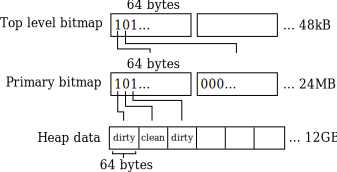
\includegraphics[width=.7\linewidth]{OLTP_design/bitset.pdf}
  \caption{\textbf{Hierarchical bitmap set.} Each bit of top level bitmap corresponds to a cache line of bits (64 bytes, 512 bits) in the primary bitmap; top level bit is set if any associated bits in primary bitmap are set (boolean \emph{or} operation).  Each bit in the primary bitmap corresponds to a cache line in the database buffer cache and is set if the cache line is dirty (contains modifications since the start of the batch).}
  \label{fig::bitset}
\end{figure}


The ideal set data structure would use an insert operation similar to the bitmap set (requiring only a bitwise-or operation) but iterate through the set faster.
I observe that at the end of each batch only a small portion of the buffer cache is dirty---set iteration should recognize large contiguous blocks of clean addresses and skip these.
The hierarchical bitmap set introduces an additional bitmap, the \emph{top level bitmap}, which indicates if an entire cache line of the \emph{primary bitmap} contains any 1s---each bit of the top level bitmap maps to 512 bits of the primary bitmap.
Figure~\ref{fig::bitset} shows the hierarchical bitmap set.
The top level bitmap (48kB) contains bits corresponding to cache lines of the primary bitmap (24MB) which in turn contains bits corresponding to cache lines of the heap (12GB buffer cache).
In the Figure the first bit of the top level bitmap is set, denoting that at least one bit in the first cache line of the primary bitmap must be set.
On the other hand, the second bit of the top level bitmap is not set, indicating that no bits in the second cache line of the primary bitmap are set, and that all corresponding cache lines in the heap are clean.

During batch execution addresses are added to the hierarchical bitmap set by setting the correct bits in both the primary and top level bitmaps.
Since bits within the same byte in the top level bitmap correspond to different heap pages, and thus must allow concurrent operations, the top level bitmap must be updated using an atomic-or instruction.
Iteration is performed by scanning the top level bitmap until a 1 is found, and then scanning the corresponding cache line of the primary bitmap.
I additionally optimize bitmap scanning by testing data at eight-byte granularity, then one-byte granularity, and then by bit.
Any block without a set bit (i.e., the block equals zero) is skipped.
Scanning at successively smaller granularity minimizes the number of instructions necessary to search the bitmap.
Processor-specific instructions enable scanning of larger data blocks, but I found additional optimization unnecessary.
Finally, the bitmaps are cleared using \emph{memset}, while clean portions of the primary bitmap may be skipped.

I map each bit of the top level bitmap to 64 bytes (512 bits) of the primary bitmap to minimize the number of cache lines accessed, but this mapping may be modified.
Additional layers of bitmaps may also be added.
These changes would depend on the access characteristics and sparseness of data within the set.
My structure appears to match my workloads and minimizes insert, iteration, and clearing overheads.

\textbf{Concurrent batch persist.}
I have shown that dirty lines can be tracked and iterated over efficiently.
However, persisting each batch with the batch coordinator alone results in long persist delays.
These delays are due to the \emph{software} overhead of copying data, not NVRAM limitations.
To reduce these delays persist operations must be parallelized across threads.
I use quiesced transaction threads, formerly waiting for the previous batch to commit, to log and persist the batch and accelerate batch commit.

The buffer cache address space and corresponding portions of the primary bitmap are partitioned into segments and placed in a task queue.
The batch coordinator and transaction threads blocked by the persist process each participate by processing tasks, persisting buffer cache partitions (both log and then data in-place).
Once all tasks complete the batch commits, allowing the next batch to begin.

\begin{table}
  \centering
  \begin{tabular}{l l}
    \hline
    Workload & Relative performance \\
    \hline \hline
    TPCC & 79.2\% \\
    TPCB & 86.2\% \\
    TATP & 83.8\% \\
    \hline
  \end{tabular}
  \caption{\textbf{Concurrent \GroupCommit persist.} \GroupCommit must use many threads to concurrently persist the batch log and data.  Here I show the relative throughput of using only a single thread versus additionally using quiesced transaction threads to accelerate batch persist and commit.  Results assume a 20ms batch period.}
  \label{table::ConcurrentPersist}
\end{table}

Table~\ref{table::ConcurrentPersist} shows the relative slowdown that results from using only a single thread to persist and commit each batch using a 20ms batch period.
At worst, 20\% throughput is lost (TPCC), yet all workloads suffer at least a 13.8\% slowdown.
Threads must persist each batch concurrently to achieve the throughput of \InPlace while remaining resilient to large persist barrier latency.

Using the hierarchical bitmap set and concurrent persist accelerates batch commit.
Profiling indicates that \emph{memcpy} operations, copies from the buffer cache to the persistent address space, form the remaining bottleneck (memcpy is implemented using fast SSE instructions and cannot be optimized further).
Persist time is minimized, with little room left for improvement.

\section{Design Space}
\label{sec:OLTP_design:Designs}
I describe the space of possible designs given choices regarding NVRAM read and write performance.
This discussion ignores possible uses of hard disk to provide additional capacity.
Each design works alongside magnetic disk with additional buffer management and the constraint that pages persist to disk before being evicted from NVRAM.
Many modern OLTP applications' working sets are small, fitting entirely in main-memory.

Table~\ref{table::DesignSpace} lists the possible combinations of caching architectures and recovery mechanisms.
The left column presents \NVDisk, the obvious and most incremental use for NVRAM.
Of note is the center-left cell, \NVDisk without the use of a volatile buffer.
WAL, by its design, allows pages to write back asynchronously from volatile storage.
Removing the volatile cache requires transactions to persist data in-place, but do so only after associated log entries persist, retaining the software overheads of \NVDisk as well as the frequent synchronization in \InPlace.
Thus, this design is impractical.

The middle-column recovery mechanism, \InPlace, represents the most intuitive use of NVRAM in database systems, as noted in several prior works.
Agrawal and Jagadish explore several algorithms for atomic durable transactions with an NVRAM main-memory \cite{AgrawalJagadish89}.
They describe the operation and correctness of each mechanism and provide an analytic cost model to compare them.
Their work represents the middle column, middle row of Table~\ref{table::DesignSpace} (\InPlace with no volatile buffer).
Aky\"{u}rek and Salem present a hybrid DRAM and NVRAM buffer cache design alongside strategies for managing cache allocation \cite{SalemAkyrek95}.
Such \emph{Partial Memory Buffers} resemble the middle-top cell of our design space table (\InPlace with a software-managed DRAM buffer), although their design considers NVRAM as part of a hybrid buffer, not the primary persistent store.
Neither of these works considers alternative approaches (such as \GroupCommit), to account for large persist barrier latency and associated delays.
Additionally, this work extends prior work by providing a more precise performance evaluation and more detailed consideration of NVRAM characteristics.

The right column presents \GroupCommit.
Each of the three recovery mechanisms may replicate all data between NVRAM and DRAM to ensure fast read accesses, manage a smaller DRAM buffer cache, or omit the cache altogether.
In Section~\ref{sec:OLTP_eval:Reads} I consider the importance of NVRAM caching to transaction throughput.
Then, in Section~\ref{sec:OLTP_eval:Persists} I assume a DRAM-replicated heap to isolate read performance from persist performance in evaluating each recovery mechanisms's ability to maximize transaction throughput.

\section{Related Work}
\label{sec:OLTP_design:RelatedWork}
To the best of my knowledge, this work is the first to investigate NVRAM write latency and its effect on durable storage and recovery in OLTP.
A large body of related work considers applications of NVRAM and reliable memories.

Ng and Chen place a database buffer cache in battery-backed DRAM, treating it as reliable memory \cite{NgChen97}.
However, the mechanisms they investigate are insufficient to provide ACID properties under any-point failure or protect against many types of failure (e.g., power loss).

Further work considers NVRAM in the context of file systems.
Baker \emph{et al.} use NVRAM as a file cache to optimize disk I/O and reduce network traffic in distributed file systems, yet continue to assume that disk provides the bulk of persisted storage \cite{BakerAsami92}.
More recently, Condit \emph{et al.} demonstrate the hardware and software design necessary to implement a file system entirely in NVRAM as the Byte-Addressable Persistent File System (BPFS) \cite{ConditNightingale09}.
While I assume similar hardware, I additionally consider a range of NVRAM performance and focus instead on databases.

Other work develops programming paradigms and system organizations for NVRAM.
Coburn \emph{et al.} propose NV-Heaps to manage NVRAM within the operating system, provide safety guarantees while accessing persistent stores, and atomically update data using copy-on-write \cite{CoburnCaulfield11}.
Volos \emph{et al.} similarly provide durable memory transactions using Software Transactional Memory (STM) and physical redo logging per transaction \cite{VolosTack11}.
While these works provide useful frameworks for NVRAM, they do not investigate the effect of NVRAM persist latency on performance, nor do they consider OLTP, where durability is tightly coupled with concurrency and transaction management.

Recently, researchers have begun to focus specifically on databases as a useful application for NVRAM.
Chen \emph{et al.} reconsider database algorithms and data structures to address NVRAM's write latency, endurance, and write energy concerns, generally aiming to reduce the number of modified NVRAM bits \cite{ChenGibbons11}.
However, their work does not consider durable consistency for transaction processing.
Venkataraman \emph{et al.} demonstrate a multi-versioned log-free B-Tree for use with NVRAM \cite{VenkataramanTolia11}.
Indexes are updated in place, similarly to my \InPlace, without requiring any logging (physical or otherwise) and while providing snap shot reads.
This work considers durability management at a higher level, user transactions, and consistency throughout the entire database.
Finally, Fang \emph{et al.} develop a new WAL infrastructure for NVRAM that leverages byte addressable and persistent access \cite{FangHsiao11}.
Fang aims to improve transaction throughput but retains centralized logging.
I distinguish myself by investigating how NVRAM write performance guides database and recovery design more generally.

More similar to my work, Coburn \emph{et al.} introduce hardware support for durable transactions in NVRAM storage devices \cite{Coburn13}.
These \emph{editable atomic writes} provide the same functionality as traditional ARIES logs.
Such hardware must still serialize and persist log entries; contention while serializing entries and ordering persists may still limit system throughput.
Finally, editable atomic writes use physical logging (updates are recorded as location-data-length tuples), as opposed to logical logging (updates are recorded as a set of data and functions to apply/roll back the update).
Logical logging is necessary to precisely control data placement in the presence of concurrent transactions.
For example, to maintain B+Tree elements in sorted order within a page each transaction may have to modify large portions of the page (to shift entries), even if those entries were recently modified by an outstanding transaction.
It is unclear if physical logging provides all the features we expect from ARIES.

%While different than byte addressable NVRAMs, Flash memory has become an important storage medium.
%Similar in theme to this work, numerous authors have considered designing databases specifically for Flash (\cite{BernsteinReid11}, \cite{SarwatMokbel11}).
%NVRAM, unlike Flash, allows more efficient in-place updates through byte-addressability, low persist latency, and atomic persists.

Prior work (e.g., H-Store \cite{StonebrakerMadden07}) has suggested highly available systems as an outright replacement for durability.
I argue that computers and storage systems will always fail, and durability remains a requirement for many applications.

\section{Conclusion}
\label{sec:OLTP_design:Conclusion}
This chapter motivated the need to reconsider system design for NVRAM recovery management.
I highlight possible caching architectures as well as three candidate recovery management software designs and their implementations.
The next chapter compares these system designs, considering performance related to NVRAM read and persist latencies.
